\documentclass{article}
\usepackage[utf8]{inputenc}
\usepackage{listings}
\usepackage{graphicx}
\usepackage{float}
\usepackage{xcolor}
\usepackage{geometry}
\usepackage{CJKutf8}
\usepackage{amsmath}
\usepackage{amssymb}

\geometry{a4paper,scale=0.8}
\lstset{
    basicstyle          =   \sffamily,        
    keywordstyle        =   \bfseries,         
    commentstyle        =   \rmfamily\itshape, 
    stringstyle         =   \ttfamily, 
    flexiblecolumns,               
    numbers             =   left,  
    showspaces          =   false, 
    showstringspaces    =   false,
    captionpos          =   t,     
    frame               =   lrtb, 
}

\lstdefinestyle{Python}{
    language        =   Python, % 语言选Python
    basicstyle      =   \zihao{-5}\ttfamily,
    numberstyle     =   \zihao{-5}\ttfamily,
    keywordstyle    =   \color{blue},
    keywordstyle    =   [2] \color{teal},
    stringstyle     =   \color{magenta},
    commentstyle    =   \color{red}\ttfamily,
    breaklines      =   true,  
    columns         =   fixed,  
    basewidth       =   0.5em,
}

\title{\bf\Large  概率论与数理统计 第6次作业}
%%%%%%%%%%%%%%%%%%%%%%%%%%%%%%%%%%%%%%
%% DON'T forget to change this part %%
\author{\bf Name: 宋昊原 \qquad Student ID: 2022010755}
%%%%%%%%%%%%%%%%%%%%%%%%%%%%%%%%%%%%%%

\begin{document}
\begin{CJK}{UTF8}{gbsn}
\maketitle
\section{泊松分布的和}
由于$X_{i}\sim P(\lambda_{i})$,我们有
$$ P(X_{i}=k)=\frac{\lambda_{i}^{k}}{k!}e^{-\lambda_{i}}$$
则
$$ P(Y=k)=\sum\limits_{i=0}^{k}P(X_{1}=i)P(X_{2}=k-i)$$
$$ =\sum\limits_{i=0}^{k}\frac{\lambda_{1}^{i}e^{-\lambda_{1}}\lambda_{2}^{k-i}e^{-\lambda^{2}}}{i!(k-i)!}$$
$$ =\sum\limits_{i=0}^{k}\frac{\tbinom{k}{i}\lambda_{1}^{i}\lambda_{2}^{k-i}}{k!}e^{-\lambda_{1}-\lambda_{2}}$$
$$ =\frac{e^{-(\lambda_{1}+\lambda_{2})}}{k!}\sum\limits_{i=0}^{k}\tbinom{k}{i}\lambda_{1}^{i}\lambda_{2}^{k-i}$$
$$ =\frac{e^{-(\lambda_{1}+\lambda_{2})}}{k!}(\lambda_{1}+\lambda_{2})^{k}$$
这证明了$Y\sim P(\lambda_{1}+\lambda_{2})$.
\section{二维随机变量换元}
写出$(X,Y)$的PDF:
$$ f(x,y)=\frac{1}{2\pi}e^{-\frac{1}{2}(x^{2}+y^{2})}$$
\subsection{}
$Z$的CDF(其中可以利用$f(x,y)$关于原点对陈的性质)
$$ G(z)=P(Z\leq z)=P(\frac{Y}{X}\leq z)=2P(\frac{Y}{X}\leq z \land X>0)=2\int_{0}^{+\infty}(\int_{-\infty}^{zx}f(x,y)dy)dx$$
求导得PDF:
$$ g(z)=\frac{d}{dz}G(z)=2\int_{0}^{+\infty}xf(x,zx)dx$$
$$ =\frac{1}{\pi}\int_{0}^{+\infty}xe^{-\frac{1}{2}x^{2}(1+z^{2})}dx$$
$$ =\frac{1}{\pi}\int_{0}^{+\infty}e^{-\frac{1}{2}x^{2}(1+z^{2})}d(\frac{1}{2}x^{2})$$
$$ =-\frac{1}{\pi(1+z^{2})}e^{-\frac{1}{2}x^{2}(1+z^{2})}|_{0}^{+\infty}$$
$$ =\frac{1}{\pi(1+z^{2})}$$
\subsection{}
这里要求$R>0$.\\
$(R,\Theta)\to(X,Y)$的函数关系已知,则
$$ g(r,\theta)=f(x(r,\theta),y(r,\theta))|\det\frac{\partial(x,y)}{\partial(r,\theta)}|$$
其中Jacobi矩阵为
$$\frac{\partial(x,y)}{\partial(r,\theta)}=
\begin{bmatrix}
    \cos\theta & -r\sin\theta\\
    \sin\theta & r\cos\theta
\end{bmatrix}$$
其行列式为
$$ \det\frac{\partial(x,y)}{\partial(r,\theta)}=r(\cos^{2}\theta+\sin^{2}\theta)=r $$
故
$$ g(r,\theta)=rf(r\cos\theta,r\sin\theta) $$
$$ =\frac{r}{2\pi}e^{-\frac{1}{2}r^{2}}$$
此PDF与$\Theta$无关,可以变量分离,故$R,\Theta$独立.
\subsection{}
$(X,Y)\to(U,V)$的映射关系是线性的. 其关系为
$$ \begin{bmatrix}x \\ y\end{bmatrix}
=\begin{bmatrix}\frac{1}{2} & \frac{1}{2}\\
    \frac{1}{2} & -\frac{1}{2}\end{bmatrix}
\begin{bmatrix}u \\ v\end{bmatrix}$$
故
$$ \det\frac{\partial(x,y)}{\partial(u,v)}=-\frac{1}{2}$$
于是
$$ g(u,v)=\frac{1}{2}f(\frac{u+v}{2},\frac{u-v}{2})$$
$$ \frac{1}{4\pi}e^{-\frac{1}{4}(u^{2}+v^{2})}$$
这可以变量分离,故$U,V$独立.
\section{独立同分布变量的最值}
先考虑$Y$的CDF,由于所有$X_{i}$独立且同分布,我们有
$$ G(y)=P(Y\leq y)=P(\max\{X_{1},...,X_{n}\}\leq y)$$
$$ =P(X_{1}\leq y\land ... \land X_{n}\leq y)$$
$$ =P(X_{1}\leq y)...P(X_{n}\leq y)$$
$$ =(F(y))^{n}$$
再考虑$Z$
$$ H(z)=P(Z\leq z)=1-P(Z>z)=1-P(\min\{X_{1},...,X_{n}\}>z)$$
$$ =1-P(X_{1}>z\land ...\land X_{n}>z)$$
$$ =1-P(X_{1}>z)...P(X_{n}>z)$$
$$ =1-(1-F(z))^{n}$$
\section{三种重要的分布}
\subsection{卡方分布}
$\chi^{2}$分布定义为$n$个独立的标准正态随机变量的平方和. 即,若
$$ Q=\sum\limits_{i=1}^{n}X_{i}^{2}, X_{i}\sim N(0,1)$$
则$Q$服从自由度为$n$的$\chi^{2}$分布,记作$Q\sim\chi^{2}(n)$.
\subsection{t分布}
设两个独立的随机变量$U,V$,若$U\sim N(0,1),V\sim\chi^{2}(p)$,则$\frac{U}{\sqrt{V/p}}$服从自由度为$p$的$t$分布.
\subsection{F分布}
设独立随机变量$X\sim\chi^{2}(m),Y\sim\chi^{2}(n)$,则$\frac{X/m}{Y/n}$服从自由度为$m,n$的$F$分布.
\section{投注}
\subsection{}
考虑A马,若其获胜,则全部1000元中50元由投注站抽走,剩余950元由投注A马的人赚取,赔率为
$$ r_{A}=\frac{950-500}{500}=\frac{9}{10}$$
同理
$$ r_{B}=\frac{950-300}{300}=\frac{13}{6}$$
$$ r_{C}=\frac{950-200}{200}=\frac{15}{4}$$
\subsection{}
$$ p_{A}=\frac{1}{1+r_{A}}=\frac{10}{19}$$
$$ p_{B}=\frac{1}{1+r_{A}}=\frac{6}{19}$$
$$ p_{C}=\frac{1}{1+r_{A}}=\frac{4}{19}$$
\subsection{}
$$ p_{A}+p_{B}+p_{C}=\frac{20}{19}>1$$
这说明投注站通过降低赔率提高了下注者对三匹马获胜的期望概率,从而保证能够获利.
\section{数字特征判断题}
\subsection{}
不正确.
\\设$X,Y\sim U(0,1)$且$X,Y$独立,则
$$ Var(XY)=E(X^{2}Y^{2})-E^{2}(XY)=E(X^{2})E(Y^{2})-E^{2}(X)E^{2}(Y)=\frac{1}{9}-\frac{1}{16}=\frac{7}{144}$$
而
$$ Var(X)Var(Y)=\frac{1}{12}\times\frac{1}{12}=\frac{1}{144}$$
\subsection{}
不正确.
\\设$X\sim B(0.4)$,则其中位数为$0$,而$E(X)=0.4$.
\section{相对期望的偏差的平方最小}
左侧等于
$$ E((X-c)^{2})=E(X^{2}-2cX+c^{2})$$
$$ =E(X^{2})-2cE(X)+c^{2}$$
右侧等于
$$ Var(X)=E(X^{2})-E^{2}(X)$$
左右相减,有
$$ E((X-c)^{2})-Var(X)=E^{2}(X)-2cE(X)+c^{2}=(E(X)-c)^{2}\geq 0$$
取等当且仅当$c=E(X)$.
\section{相对中位数的偏差的绝对值最小}
左侧等于
$$E(|X-c|)=\int_{-\infty}^{c}(c-x)f(x)dx+\int_{c}^{+\infty}(x-c)f(x)dx$$
$$ =c\int_{-\infty}^{c}f(x)dx-\int_{-\infty}^{c}xf(x)dx+\int_{c}^{+\infty}xf(x)dx-c\int_{c}^{+\infty}f(x)dx$$
右侧等于
$$E(|X-m|)=\int_{-\infty}^{m}(m-x)f(x)dx+\int_{m}^{+\infty}(x-m)f(x)dx$$
$$ =\int_{-\infty}^{m}mf(x)dx-\int_{-\infty}^{m}xf(x)dx+\int_{m}^{+\infty}xf(x)dx-\int_{m}^{+\infty}mf(x)dx$$
$$ =\frac{1}{2}m-\int_{-\infty}^{m}xf(x)dx+\int_{m}^{+\infty}xf(x)dx-\frac{1}{2}m$$
$$ =-\int_{-\infty}^{m}xf(x)dx+\int_{m}^{+\infty}xf(x)dx$$
作差
$$E(|X-c|)-E(|X-m|)=c\int_{-\infty}^{c}f(x)dx-c\int_{c}^{+\infty}f(x)dx+\int_{c}^{m}xf(x)dx+\int_{c}^{m}xf(x)dx$$
$$ =c(\int_{-\infty}^{c}f(x)dx-\int_{c}^{+\infty}f(x)dx)+2\int_{c}^{m}xf(x)dx$$
$$ =c(\int_{-\infty}^{c}f(x)dx-\int_{-\infty}^{m}f(x)dx-\int_{c}^{+\infty}f(x)dx+\int_{m}^{+\infty}f(x)dx)+2\int_{c}^{m}xf(x)dx$$
$$ =-2c\int_{c}^{m}f(x)dx+2\int_{c}^{m}xf(x)dx$$
由积分第一中值定理
$$\exists\xi\ between\ c\ and\ m\ s.t. \int_{c}^{m}xf(x)dx=\xi\int_{c}^{m}f(x)dx$$
实际上这里$\xi$对应的是$X$在$c$和$m$之间部分的期望.
\\于是差值化为
$$2(\xi-c)\int_{c}^{m}f(x)dx$$
若$c\geq m$,则积分和$\xi-c$都非正,差值非负.
\\若$c<m$,则积分和$\xi-c$都非负,差值非负.
\section{对数正态分布的期望和方差}
设$Y\sim N(\mu,\sigma^{2})$,$\ln X=Y$,设$Y$的PDF为$f(y)$.
\subsection{期望}
$$ E(X)=E(e^{Y})=\int_{-\infty}^{+\infty}e^{y}f(y)dy$$
$$ =\int_{-\infty}^{+\infty}\frac{e^{y}}{\sqrt{2\pi}\sigma}\exp(-\frac{(y-\mu)^{2}}{2\sigma^{2}})dy$$
$$ =\frac{1}{\sqrt{2\pi}\sigma}\int_{-\infty}^{+\infty}\exp(-\frac{(y-\mu)^{2}-2\sigma^{2}y}{2\sigma^{2}})dy$$
$$ =\frac{1}{\sqrt{2\pi}\sigma}\int_{-\infty}^{+\infty}\exp(-\frac{y^{2}-2(\mu+\sigma^{2})y+\mu^{2}}{2\sigma^{2}})dy$$
$$ =\frac{1}{\sqrt{2\pi}\sigma}\int_{-\infty}^{+\infty}\exp(-\frac{(y-(\mu+\sigma^{2}))^{2}-2\mu\sigma^{2}-\sigma^{4}}{2\sigma^{2}})dy$$
$$ =\frac{e^{\mu+\frac{1}{2}\sigma^{2}}}{\sqrt{\pi}}\int_{-\infty}^{+\infty}\exp(-(\frac{y-(\mu+\sigma^{2})}{\sqrt{2}\sigma})^{2})d(\frac{y-(\mu+\sigma^{2})}{\sqrt{2}\sigma})$$
$$ =e^{\mu+\frac{1}{2}\sigma^{2}}$$
\subsection{方差}
$$ E(X^{2})=E(e^{2Y})=\int_{-\infty}^{+\infty}e^{2y}f(y)dy$$
$$ =\int_{-\infty}^{+\infty}\frac{e^{2y}}{\sqrt{2\pi}\sigma}\exp(-\frac{(y-\mu)^{2}}{2\sigma^{2}})dy$$
$$ =\frac{1}{\sqrt{2\pi}\sigma}\int_{-\infty}^{+\infty}\exp(-\frac{(y-\mu)^{2}-4\sigma^{2}y}{2\sigma^{2}})dy$$
$$ =\frac{1}{\sqrt{2\pi}\sigma}\int_{-\infty}^{+\infty}\exp(-\frac{y^{2}-2(\mu+2\sigma^{2})y+\mu^{2}}{2\sigma^{2}})dy$$
$$ =\frac{1}{\sqrt{2\pi}\sigma}\int_{-\infty}^{+\infty}\exp(-\frac{(y-(\mu+2\sigma^{2}))^{2}-4\mu\sigma^{2}-4\sigma^{4}}{2\sigma^{2}})dy$$
$$ =\frac{e^{2\mu+2\sigma^{2}}}{\sqrt{\pi}}\int_{-\infty}^{+\infty}\exp(-(\frac{y-(\mu+2\sigma^{2})}{\sqrt{2}\sigma})^{2})d(\frac{y-(\mu+2\sigma^{2})}{\sqrt{2}\sigma})$$
$$ =e^{2\mu+2\sigma^{2}}$$
故
$$ Var(X)=E(X^{2})-E^{2}(X)=e^{2\mu+2\sigma^{2}}-e^{2\mu+\sigma^{2}}$$
\section{样本与随机变量的数字特征}
\subsection{样本均值的方差}
$$ E(\bar{X})=\frac{1}{n}\sum\limits_{i=1}^{n}E(X_{i})=\frac{1}{n}n\mu=\mu$$
$$ E(\bar{X}^{2})=\frac{1}{n^{2}}\sum\limits_{i=1}^{n}E(X_{i}^{2})+\frac{2}{n^{2}}\sum\limits_{1\leq i<j\leq n}E(X_{i}X_{j})$$
$$ =\frac{1}{n^{2}}\sum\limits_{i=1}^{n}(Var(X_{i})+E^{2}(X_{i}))+\frac{2}{n^{2}}\sum\limits_{1\leq i<j\leq n}E(X_{i})E(X_{j})$$
$$ =\frac{1}{n^{2}}n(\sigma^{2}+\mu^{2})+\frac{2}{n^{2}}\frac{n(n-1)}{2}\mu^{2}$$
$$ =\frac{1}{n}\sigma^{2}+\mu^{2}$$
故
$$ Var(\bar{X})=E(\bar{X}^{2})-E^{2}(\bar{X})=\frac{1}{n}\sigma^{2}$$
\subsection{样本方差的期望}
$$ E(S^{2})=\frac{1}{n-1}\sum\limits_{i=1}^{n}(E(X_{i}^{2})-2E(X_{i}\bar{X})+E(\bar{X}^{2}))$$
$$ =\frac{1}{n-1}(\sum\limits_{i=1}^{n}(Var(X_{i})+E^{2}(X_{i}))-2E(\bar{X}\sum\limits_{i=1}^{n}X_{i})+n(\frac{1}{n}\sigma^{2}+\mu^{2}))$$
$$ =\frac{1}{n-1}(n\sigma^{2}+n\mu^{2}-2nE(\bar{X}^{2})+\sigma^{2}+n\mu^{2})$$
$$ =\frac{1}{n-1}(n\sigma^{2}+n\mu^{2}-\sigma^{2}-n\mu^{2})$$
$$ =\sigma^{2}$$
\section{不相关性的等价描述}
设$E(X)=\mu_{1},E(Y)=\mu_{2},Var(X)=\sigma_{1}^{2},Var(Y)=\sigma_{2}^{2}$,则四个描述在$\sigma_{1}\sigma_{2}\neq 0$时等价. 下面进行证明
\subsection{$(1)\Leftrightarrow(2)$}
$$ Cov(X,Y)=0$$
$$ \Leftrightarrow \frac{Cov(X,Y)}{\sigma_{1}\sigma_{2}}=0$$
$$ \Leftrightarrow Corr(X,Y)=0$$
这是$X,Y$不相关的定义.
\subsection{$(1)\Leftrightarrow(3)$}
$$ E(XY)=E((X-\mu_{1})(Y-{\mu_{2}})+\mu_{1}Y+\mu_{2}X-\mu_{1}\mu_{2})$$
$$ =E((X-\mu_{1})(Y-\mu_{2}))+\mu_{1}E(Y)+\mu_{2}E(X)-\mu_{1}\mu_{2}$$
$$ =Cov(X,Y)+\mu_{1}\mu_{2}$$
而
$$ E(X)E(Y)=\mu_{1}\mu_{2}$$
故
$$ E(XY)=E(X)E(Y)$$
$$ \Leftrightarrow Cov(X,Y)+\mu_{1}\mu_{2}=\mu_{1}\mu_{2}$$
$$ \Leftrightarrow Cov(X,Y)=0$$
\subsection{$(3)\Leftrightarrow(4)$}
$$ Var(X+Y)=E((X+Y)^{2})-E^{2}(X+Y)$$
$$ =E(X^{2}+2XY+Y^{2})-E^{2}(X)-2E(X)(Y)-E^{2}(Y)$$
$$ =E(X^{2})-E^{2}(X)+2E(XY)-2E(X)E(Y)+E(Y^{2})-E^{2}(Y)$$
$$ =Var(X)+Var(Y)-2(E(XY)-E(X)E(Y))$$
于是
$$ Var(X+Y)=Var(X)+Var(Y)$$
$$ \Leftrightarrow E(XY)=E(X)E(Y)$$
\section{$\rho$是相关系数}
$$ f(x,y)=\frac{1}{2\pi\sigma_{1}\sigma_{2}\sqrt{1-\rho^{2}}}\exp{(-\frac{1}{2(1-\rho^{2})}((\frac{x-\mu_{1}}{\sigma_{1}})^{2}+(\frac{y-\mu_{2}}{\sigma_{2}})^{2}-2\rho\frac{(x-\mu_{1})(y-\mu_{2})}{\sigma_{1}\sigma_{2}}))}$$
$$ Corr(X,Y)=E(\frac{X-\mu_{1}}{\sigma_{1}}\frac{Y-\mu_{2}}{\sigma-{2}})$$
$$ =\iint_{\mathbb{R}^{2}}\frac{x-\mu_{1}}{\sigma_{1}}\frac{y-\mu_{2}}{\sigma_{2}}f(x,y)dxdy$$
令$\xi=\frac{x-\mu_{1}}{\sigma_{1}}$,$\eta=\frac{y-\mu_{2}}{\sigma_{2}}$,则
$$ Corr(X,Y)=\iint_{\mathbb{R}^{2}}\frac{\xi\eta}{2\pi\sqrt{1-\rho^{2}}}\exp(-\frac{\xi^{2}+\eta^{2}-2\rho\xi\eta}{2(1-\rho^{2})})d\xi d\eta$$
令
$$ A=\begin{bmatrix}1 & -\rho \\ -\rho & 1\end{bmatrix}$$
则
$$ \xi^{2}+\eta^{2}-2\rho\xi\eta=\begin{bmatrix}\xi & \eta\end{bmatrix}A\begin{bmatrix}\xi \\ \eta \end{bmatrix}$$
对$A$做Cholesky分解,有
$$ L=\begin{bmatrix}\sqrt{1-\rho^{2}}&\\-\rho&1\end{bmatrix},A=L^{T}L$$
于是,令
$$ \alpha=\sqrt{1-\rho^{2}}\xi,\ \beta=-\rho\xi+\eta$$
就有
$$ \begin{bmatrix}\alpha\\\beta\end{bmatrix}=L\begin{bmatrix}\xi\\\eta\end{bmatrix}$$
故
$$ \xi^{2}+\eta^{2}-2\rho\xi\eta=\alpha^{2}+\beta^{2}$$
由于
$$ \det\frac{\partial(\xi,\eta)}{\partial(\alpha,\beta)}=\frac{1}{\det\frac{\partial(\alpha,\beta)}{\partial(\xi,\eta)}}=\frac{1}{\det L}=\frac{1}{\sqrt{1-\rho^{2}}}$$
且
$$ \xi=\frac{\alpha}{\sqrt{1-\rho^{2}}},\ \eta=\frac{\rho\alpha}{\sqrt{1-\rho^{2}}}+\beta$$
我们有
$$ Corr(X,Y)=\iint_{\mathbb{R}^{2}}\frac{\alpha(\rho\alpha+\sqrt{1-\rho^{2}}\beta)}{2\pi(1-\rho^{2})^\frac{3}{2}}\exp(-\frac{\alpha^{2}+\beta^{2}}{2(1-\rho^{2})})\frac{1}{\sqrt{1-\rho^{2}}}d\alpha d\beta$$
$$ =\int_{-\infty}^{+\infty}\frac{\alpha}{2\pi(1-\rho^{2})^{2}}(\int_{-\infty}^{+\infty}(\rho\alpha+\sqrt{1-\rho^{2}}\beta)\exp(-\frac{\alpha^{2}+\beta^{2}}{2(1-\rho^{2})})d\beta)d\alpha$$
$$ =\int_{-\infty}^{+\infty}\frac{\alpha\exp(-\frac{\alpha^{2}}{2(1-\rho^{2})})}{\sqrt{2}\pi(1-\rho^{2})^{\frac{3}{2}}}(\rho\alpha\int_{-\infty}^{+\infty}\exp(-(\frac{\beta}{\sqrt{(2(1-\rho^{2}))}})^{2})d(\frac{\beta}{\sqrt{2(1-\rho^{2})}})$$
$$+\sqrt{2}(1-\rho^{2})\int_{-\infty}^{+\infty}\frac{\beta}{\sqrt{2(1-\rho^{2})}}\exp(-(\frac{\beta}{\sqrt{2(1-\rho^{2})}})^{2})d(\frac{\beta}{\sqrt{2(1-\rho^{2})}}))d\alpha$$
$$=\int_{-\infty}^{+\infty}\frac{\alpha\exp(-\frac{\alpha^{2}}{2(1-\rho^{2})})}{\sqrt{2}\pi(1-\rho^{2})^{\frac{3}{2}}}(\sqrt{\pi}\rho\alpha+0)d\alpha$$
$$=\frac{\rho}{\sqrt{2\pi}(1-\rho^{2})^{\frac{3}{2}}}\int_{-\infty}^{+\infty}\alpha^{2}\exp(-\frac{\alpha^{2}}{2(1-\rho^{2})})d\alpha$$
$$=\frac{2\rho}{\sqrt{\pi}}\int_{-\infty}^{+\infty}(\frac{\alpha}{\sqrt{2(1-\rho^{2})}})^{2}\exp(-(\frac{\alpha}{\sqrt{2(1-\rho^{2})}})^{2})d(\frac{\alpha}{\sqrt{2(1-\rho^{2})}})$$
$$=\rho$$
\section{配对问题的期望与方差}
用$X_{i}$表示第$i$个人拿到自己的帽子的情况,拿到为1,没拿到为0;$X$表示拿到自己帽子的人数,则
$$ X=\sum\limits_{i=1}^{n}X_{i}$$
$$ E(X_{i})=\frac{1}{n}$$
\subsection{期望}
$$ E(X)=\sum\limits_{i=1}^{n}E(X_{i})=1$$
\subsection{方差}
$$ E(X^{2})=\sum\limits_{i=1}^{n}E(X_{i}^{2})+2\sum\limits_{1\leq i<j\leq n}E(X_{i}X_{j})$$
由于
$$ E(X_{i}^{2})=\frac{1}{n}$$
$$ E(X_{i}X_{j})=\frac{1}{n(n-1)}$$
故
$$ E(X^{2})=n\frac{1}{n}+2\tbinom{n}{2}\frac{1}{n(n-1)}=2$$
故
$$ Var(X)=E(X^{2})-E^{2}(X)=1$$
\section{Cauchy-Schwarz不等式}
\subsection{}
先考虑$E(V^{2})=0$时,此时$P(V=0)=1$,不等式两边都是0,且存在$c=0$时$P(V=cU)=1$,故成立.
\\\\
再考虑$E(V^{2})>0$时
$$ E((U-tV)^{2})=E(U^{2})-2E(UV)t+E(V^{2})t^{2}\geq 0$$
这是关于$t$的二次项系数为正的的二次函数,故
$$ 4E^{2}(UV)-4E(U^{2})E(V^{2})\leq 0$$
即
$$ E^{2}(UV)\leq E(U^{2})E(V^{2})$$
此时等号成立等价于上述二次函数与$t$轴相切,即
$$ \exists t_{0}\in\mathbb{R},\ E((U-t_{0}V)^{2})=0$$
这意味着
$$ P(U=t_{0}V)=1$$
若$t_{0}=0$,则$P(U=0)=1$,这相当于最开始讨论的情形,下面假设$t_{0}\neq 0$.\\
取$c=\frac{1}{t_{0}}$则有
$$ P(V=cU)=1$$
\subsection{}
设$E(X)=\mu_{1},E(Y)=\mu_{2},Var(X)=\sigma_{1}^{2},Var(Y)=\sigma_{2}^{2}$,则
$$ Corr(X,Y)^{2}=E^{2}(\frac{X-\mu_{1}}{\sigma_{1}}\frac{Y-\mu_{2}}{\sigma_{2}})$$
$$ \leq E((\frac{X-\mu_{1}}{\sigma_{1}})^{2})E((\frac{Y-\mu_{2}}{\sigma_{2}})^{2})=1$$
故$|Corr(X,Y)|\leq 1$,且等号成立当且仅当
$$\exists c\ s.t.\ P(\frac{Y-\mu_{2}}{\sigma_{2}}=c\frac{X-\mu_{1}}{\sigma_{1}})=1$$
上述概率的条件等价于
$$ Y=\frac{c\sigma_{2}}{\sigma_{1}}X-\frac{\mu_{1}\sigma_{2}}{\sigma_{1}}+\mu_{2}$$
取
$$ a=\frac{c\sigma_{2}}{\sigma_{1}},\ b=-\frac{\mu_{1}\sigma_{2}}{\sigma_{1}}+\mu_{2}$$
即可.
\section{独立同分布随机变量的进一步讨论}
\subsection{}
$$ Cov(X_{i}-\bar{X},\bar{X})=E((X_{i}-\bar{X})(\bar{X}-\mu))$$
$$ =E(X_{i}\bar{X})-E(\bar{X}^{2})-\mu E(X_{i})+\mu E(\bar{X})$$
$$ =\frac{1}{n}\sum\limits_{j=1}^{n}E(X_{i}X_{j})-\frac{1}{n^{2}}(\sum\limits_{j=1}^{n}E(X_{j}^{2})+2\sum\limits_{1\leq j<k\leq n}E(X_{j}X_{k}))-\mu^{2}+\mu^{2}$$
$$ =\frac{n-1}{n}\mu^{2}+\frac{1}{n}(\mu^{2}+\sigma^{2})-\frac{1}{n^{2}}n(\mu^{2}+\sigma^{2})-\frac{2}{n^{2}}\frac{n(n-1)}{2}\mu^{2}$$
$$ =0$$
\subsection{}
不一定独立,反例如下:
\\\\设$X_{1},X_{2}\sim B(\frac{1}{2})$,则
$$ P(X_{1}-\bar{X}=0)=P(X_{1}=X_{2})=\frac{1}{2}$$
$$ P(X_{1}-\bar{X}=0|\bar{X}=\frac{1}{2})=0$$
\section{计算机实验:Q-Q图验证正态性}
\subsection{}
\begin{minipage}{0.5\textwidth}
    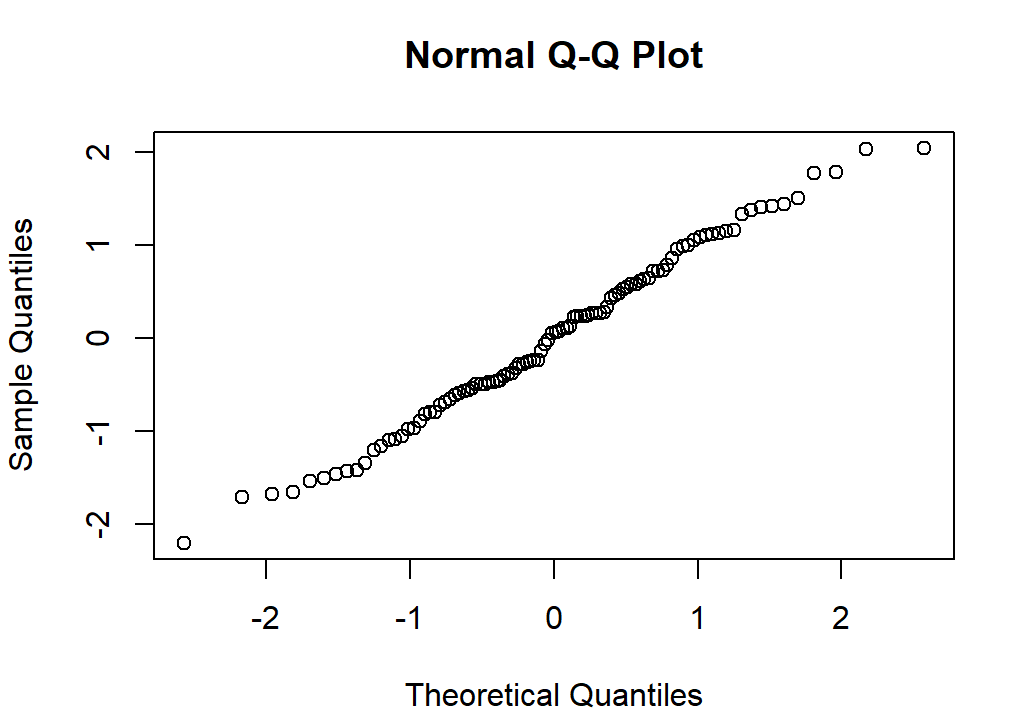
\includegraphics[scale=0.6]{qqplot_norm.png}
\end{minipage}
\subsection{}
\begin{minipage}{0.5\textwidth}
    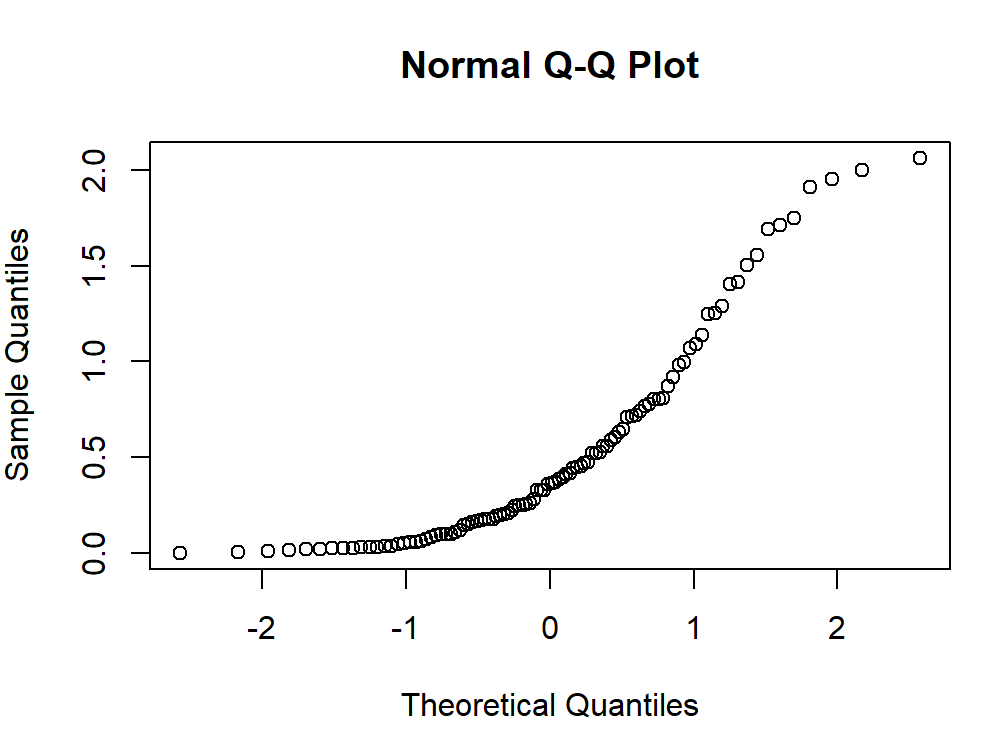
\includegraphics[scale=0.6]{qqplot_exp.png}
\end{minipage}
\subsection{}
可以,只要把$\Phi^{-1}$改为指定分布的CDF的反函数即可.
\subsection{}
可以,只要把两组数据都从小到大排列后一个作为$x$轴一个作为$y$轴作图即可,这可以使用R语言中的qqplot函数完成.
\subsection{使用的代码}
\begin{minipage}{0.5\textwidth}
    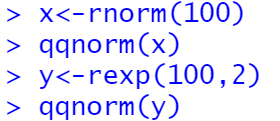
\includegraphics[scale=0.6]{code.png}
\end{minipage}
\end{CJK}
\end{document}